The experimental design is structured to answer three empirical questions. First, how difficult is the forecasting problem once HAR is treated as a serious baseline rather than as a placeholder comparator? Second, does the proposed multiscale representation add value uniformly, or only under specific horizons, targets, and market states? Third, does the spillover layer contribute incremental predictive information beyond within-index wavelet features? Every component of the evaluation protocol is chosen to answer these questions under a strict no-leakage standard.

\subsection{Walk-Forward Protocol}

All experiments follow a rolling walk-forward protocol. Each model is estimated on a fixed window of 1260 trading days (approximately five calendar years). After generating the out-of-sample forecast, the evaluation origin advances by one trading day. The evaluation period runs from 4 January 2016 to 31 December 2025, yielding 2513 out-of-sample steps in the main experiment. To reduce unnecessary computational noise while preserving chronology, model refitting is scheduled every five trading days within the rolling process.

\begin{figure}[!t]
\centering
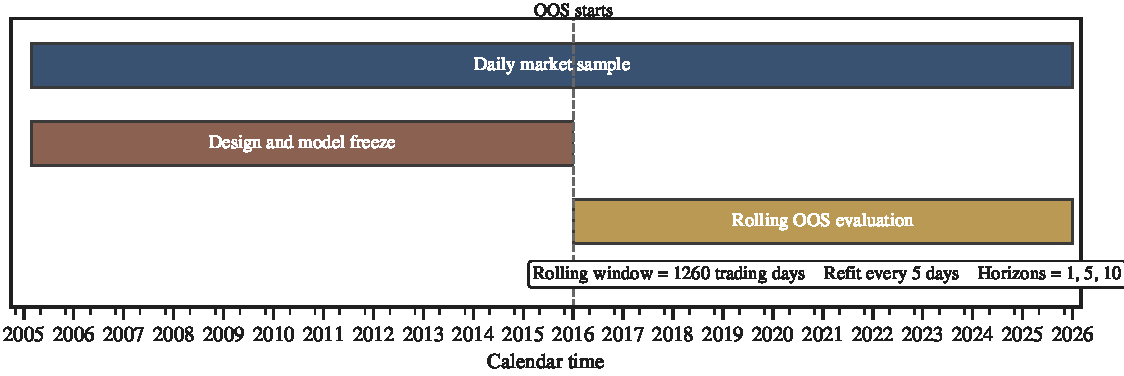
\includegraphics[width=0.96\textwidth]{figures/fig09_protocol_timeline.pdf}
\caption{Rolling walk-forward evaluation protocol. Each step advances the forecast origin by one trading day. The training window (1260 days, shaded) rolls forward to generate the out-of-sample forecast sequence spanning 2016--2025. All feature construction, model fitting, warning-threshold calibration, and evaluation are performed strictly within the boundary of each training window, ensuring full causal integrity.}
\label{fig:protocol_timeline}
\end{figure}

Figure~\ref{fig:protocol_timeline} illustrates the rolling evaluation structure. The causality requirement applies to the full pipeline, not only to the final model fit. Feature standardization, clipping rules, wavelet decomposition, threshold estimation, calibration floors, and warning thresholds are all computed strictly within the current training window. No full-sample preprocessing is used at any stage. This point is crucial because modest-looking violations of chronology, especially in feature construction or normalization, can materially exaggerate out-of-sample performance in financial machine-learning studies.

\subsection{Forecast Horizons, Benchmarks, and Evaluation Metrics}

The main forecast horizons are \(h=1\), \(h=5\), and \(h=10\), corresponding to one trading day, one trading week, and approximately two trading weeks. These horizons separate the short-run persistence problem from the medium-horizon risk-monitoring problem. If a proposed method cannot compete at \(h=1\), that is informative. If it becomes more competitive at \(h=5\) and \(h=10\), that suggests it is capturing slower-moving structure that HAR alone cannot fully absorb.

The benchmark set is intentionally demanding. It includes naive historical-volatility baselines, HAR, raw LightGBM, and wavelet-enhanced LightGBM, as well as the spillover-augmented extension. Additional machine-learning and deep-learning baselines are included so that any performance gain can be attributed to multiscale feature design rather than to model capacity alone.

The primary regression metric is QLIKE because it is widely used in volatility forecasting and is sensitive to both prediction error and scale miscalibration for positive targets \cite{patton2011proxy}. RMSE, MAE, and out-of-sample \(R^2\) are reported as supporting metrics. The out-of-sample coefficient of determination is defined as
\[
R^2_{OOS}
=
1-
\frac{\sum_t (y_t-\hat y_t)^2}
{\sum_t (y_t-\hat y_t^{\,bench})^2}.
\]
For the warning task, PR-AUC is the primary metric because the high-volatility class is intentionally rare under the rolling 90th-percentile rule. ROC-AUC, Brier score, precision, and recall are reported as complementary measures. The Brier score is
\[
\text{Brier}
=
\frac{1}{T}\sum_{t=1}^{T}(p_t-z_t)^2,
\]
where \(p_t\) is the predicted warning probability and \(z_t\) is the realized event label. The threshold-dependent warning quantities are
\[
\text{Precision}(c)=\frac{TP(c)}{TP(c)+FP(c)},
\qquad
\text{Recall}(c)=\frac{TP(c)}{TP(c)+FN(c)},
\]
and
\[
F_{\beta}(c)=
\frac{(1+\beta^2)\,\text{Precision}(c)\,\text{Recall}(c)}
{\beta^2\,\text{Precision}(c)+\text{Recall}(c)}.
\]
The operating threshold for the logistic warning model is chosen by maximizing \(F_2\), reflecting the fact that missed high-volatility episodes are typically more costly than additional false alarms in applied risk surveillance \cite{saito2015prauc}.

\subsection{Three-Step Ablation Design}
\label{subsec:ablation_design}

The core methodological claim of the paper is evaluated through a three-step ablation ladder:

\begin{description}[leftmargin=2.6em, style=nextline]
\item[Step~1: HAR $\to$ Wavelet-LGB]
This comparison tests whether within-index multiscale representation adds predictive value beyond a strong persistence benchmark. It asks whether scale-specific information from the target index's own history contains useful signal beyond the standard 1-, 5-, and 22-day persistence aggregates.

\item[Step~2: Wavelet-LGB $\to$ Spillover-LGB]
This is the central test of the Cross-Index Wavelet Spillover Hypothesis. The only difference between the two models is the addition of the spillover block \(\bm{\phi}_{k\to i,t}\). Any improvement observed here is therefore attributable specifically to peer-index frequency-domain information.

\item[Full gap: HAR $\to$ Spillover-LGB]
This comparison summarizes the cumulative effect of moving from a pure persistence benchmark to the full CMWSL representation.
\end{description}

The value of this ladder is that it prevents the paper from making vague claims about hybrid modelling. Each modelling increment has an identifiable information interpretation: persistence, within-index multiscale representation, and cross-index spillover.

\subsection{Statistical Inference}

Each index--horizon cell is evaluated with explicit out-of-sample forecast comparison tests. The Diebold--Mariano (DM) test is used for non-nested comparisons \cite{diebold1995predictive}. The Clark--West (CW) test is used as the primary inferential tool when the larger model nests the smaller one \cite{clark2007nested}. In the present design, Step~1 is treated with DM because the comparison is conceptually between different representation families, while Step~2 is explicitly nested and therefore primarily evaluated with CW. Reporting both tests increases transparency, but CW is the correct test for the spillover claim because it adjusts for the parameter-estimation noise introduced by the extra regressors.

The DM test is implemented as a two-tailed Newey--West HAC procedure with lag \(\lfloor T^{1/3}\rfloor\). The CW test is implemented one-tailed with the larger model as model \(b\), matching the directional hypothesis that spillover information should improve, rather than simply alter, predictive performance. The nine index--horizon cells are reported separately. No multiple-testing correction is imposed because the spillover analysis is not presented as an exploratory search over arbitrary cells; it is a pre-specified directional test with full cell-level disclosure in Table~\ref{tab:spillover_ablation}.

\subsection{Robustness Strategy}

Two robustness designs are used to test whether the main findings survive beyond one carefully selected benchmark environment. The first augments the predictor set with a broader block of public risk indicators---credit spreads, policy uncertainty variables, and term-structure signals---asking whether multiscale representation becomes more useful in a richer, stress-aligned environment. The second substitutes the Parkinson estimator for the Rogers--Satchell target, asking whether model rankings change when the volatility proxy draws more heavily on OHLC range information.

Together, these designs provide a stronger standard than a single-sample comparison. A method that performs well only under one volatility proxy and one feature set is difficult to generalize. A method whose relative advantage becomes visible precisely when the information environment is richer, or when the target contains stronger OHLC range information, offers a more credible contribution to risk forecasting.
